\documentclass{article}
\usepackage[utf8]{inputenc}
\usepackage{amsmath}
\usepackage{graphicx}
\usepackage{setspace}
\usepackage{mathtools}
\usepackage{subfig}
\usepackage{caption}
\usepackage{placeins}
\usepackage{multirow}
\usepackage{longtable}
\usepackage{indentfirst}
\usepackage{wrapfig}
\usepackage{chemfig}

%Paragraph jumps and indentation
\setlength{\parskip}{1.6em}
\setlength{\parindent}{1.25cm}
%Border
\usepackage[left=1in, right=1in, top=1in, bottom=1in]{geometry}

\begin{document}
\begin{center}
    \par{\huge \textbf{The Effect of Organic and Inorganic Salts on Surface Tension of Water}}
\end{center}


\section{Introduction}

\par{The surface tension of a material is an important property of a material with many applications in our lives from the low surface tension in antiseptics allowing for quick spreading of it over a wound to the high surface tension of water enabling water-striding insects to 'run' on water. My interest in surface tension began after seeing a video of the plumed basilisk lizard running on water. I was surprised that a relatively heavy body like the lizard, which is also denser than water, was able to glide across water easily and wanted to investigate factors, specifically chemical additions, that would manipulate surface tension, so that heavier bodies could also glide across water or other liquid surfaces.}

\par{Surface tension ($\sigma$) is defined as the energy, or work, required to increase the surface area of
a liquid due to inter-molecular forces.\footnote{Petrucci, Ralph H., et al. General Chemistry: Principles and Modern Applications. Upper Saddle River, NJ: Prentice Hall, 2017} It can be modelled by the following equation:}

\begin{equation}
    \sigma = \frac{\text{Energy}}{\text{Surface~Area}}
\end{equation}

\par{These inter-molecular forces depend on the nature of the liquid and, thus, each liquid exhibits different surface tensions. Additionally, as the inter-molecular forces of a liquid are dependent on the solutes, a solution of a liquid solvent and solute would have different surface tensions. Due to the surface tension being constant at fixed values, the ratio of mass to surface tension for liquids is also constant:}

\begin{equation}
    \frac{m_1}{\sigma_1} = \frac{m_2}{\sigma_2}
\end{equation}

\par{\large \textbf{A Molecular Perspective}}

\begin{figure}[!h]
\centering
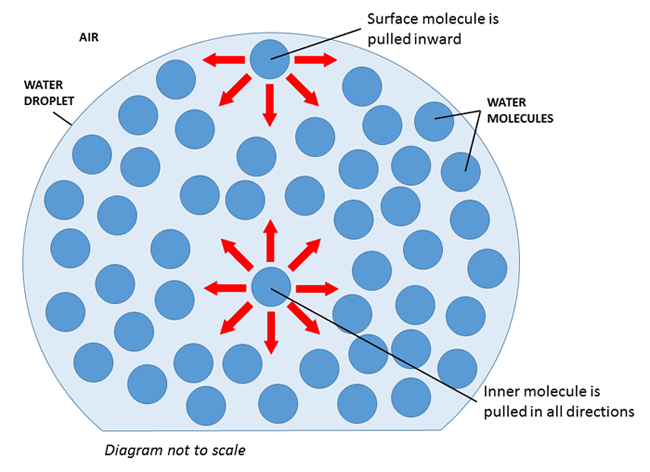
\includegraphics[width=5.5cm]{Surface tension.png}
\caption{Water molecules at the surface experience a net attractive force to neighbouring molecules, holding the surface together. The interior molecules experience a uniform attractive force.\protect\footnotemark{}}\label{wrap-fig:1}
\end{figure} 

\footnotetext{Science Buddies. “Measuring Surface Tension of Water with a Penny | Science Project.” Science Buddies, 20 Nov. 2020, www.sciencebuddies.org/science-fair-projects/project-ideas/Chem$\texttt{\_}$p021/chemistry/measuring-surface-tension-of-water-with-a-penny$\texttt{\#}$background.}

\par {There exist two kinds of particles in any fluid (figure 1): particles on the inside of the fluid, interior particles, and particles on the boundary of the fluid, exterior particles. Since the interior particles are attracted to all the particles around them, while exterior particles are only attracted to other exterior particles and interior particles directly below them, interior particles have a lower energy state than exterior particles. This results in the particles maintaining a minimum surface area to have more particles in a lower energy state, resulting in surface tension. Inter-molecular forces (such London dispersion forces or Van der Waals forces) exist between liquids and are responsible for the surface tension. It takes energy to break these forces and, thus, the surface tension. This is the reason why water has a high surface tension value. Because of it's strong hydrogen bonds, it requires a great amount of energy to break these bonds and overcome the surface tension of water.}

\section{Design}

\subsection{Research Question}

\par{How does the addition of inorganic or organic salts affect the surface tension of water?}

\subsection{Hypothesis}

\par{The addition of organic salts would decrease surface tension ($\sigma$) of water and the addition of inorganic salts would increase the surface tension ($\sigma$) of water. Because of water's charge, a water molecule would bind more strongly to the inorganic salt's ions, which would increase the strength of the network of inter-molecular bonds of water. Contrary to this, as the organic salts are absorbed they would break the strong polar bonds between water molecules and because the inter-molecular force between water and an organic molecules is weaker than the polar bond between two water molecules. If $\sigma$ is plotted against the different salts used, all other things held constant, the greatest y-coordinate would be produced for the aqueous inorganic salt solutions, an intermediary y-coordinate would be produced for distilled water and the smallest y-coordinate would be produced by the organic salts.}

\subsection{Variables}

\begin{spacing}{2}
    \par{\vspace{-0.5cm} \hspace{-1.4cm}
    \textbf{A. Independent Variable:} Aqueous Salt
    \newline
    \textbf{B. Dependent Variable:} Surface Tension of Liquid ($\textt{\sigma}$) 
    \newline
    \textbf{C. Control Variables:} \newline
   \hspace*{0.5cm} \textbf{I. }Temperature of the liquid \newline}
\end{spacing}

\hfill\begin{minipage}{\dimexpr\textwidth-1cm}
\vspace{-1.3cm}
\par{\textbf{a) Reason:} Surface tension of a liquid decreases with an increase in temperature because the increase in molecular thermal activity causes a decrease in the cohesive, inter-molecular forces. \footnotemark \protect   \newline \newline
\textbf{b) Method:} The experiment was conducted in a water bath at an ambient temperature of 35°C}
\xdef\tpd{\the\prevdepth}
\end{minipage}

\footnotetext{Bustos, Elsa Susana Sepúlveda. “Surface Tension.” Surface Tension and Capillarity, University of Florida, 2004,  fsz.ifas.ufl.edu/surfacetensionandcapillarity/html/en$\_$tension.htm}

\begin{spacing}{1}
    \hspace{-0.8cm}
    \textbf{II. }Concentration of salts
\end{spacing}

\hfill\begin{minipage}{\dimexpr\textwidth-1cm}
\par{\textbf{a) Reason:}Different concentration of salts would affect the surface tension of water drastically and differently as they would result in different inter-molecular forces.  \newline \newline
\textbf{b) Method:}The concentration of salts was kept constant at 1 mole/Litre (mol/L) \newline}
\xdef\tpd{\the\prevdepth}
\end{minipage}

\subsection{Apparatus}

\begin{enumerate}
    \item Clamp-stand
    \item Stalagmometer
    \item Weighing Balance
    \item Gravity Bottle
    \item Beaker
    \item Stirring Rod
    \item Spatula
    \item Various organic and inorganic salts: Lithium Sulphate ($\textt{Li_{2}SO_{4}}$), Sodium Sulphate ($\textt{Na_{2}SO_{4}}$), Potassium Sulphate ($\textt{K_{2}SO_{4}}$), Beryllium Sulphate ($BeSO_{4}$), Magnesium Sulphate ($MgSO_{4}$), Calcium Sulphate ($CaSO_{4}$), Sodium Acetate ($CH_{3}COONa$), Potassium Acetate ($CH_{3}COOK$)
\end{enumerate}

\begin{figure}[!h]
    \centering
    \subfloat[\centering Side 1]{{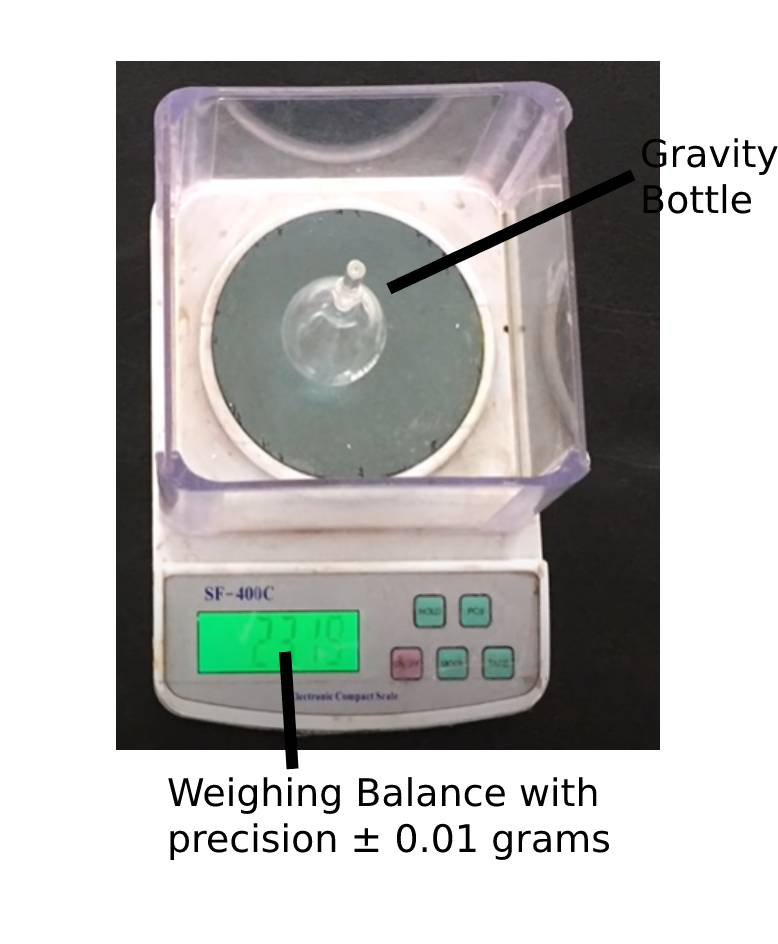
\includegraphics[width=5cm]{New Project (1).jpg} }}%
    \qquad
    \subfloat[\centering Side 2]{{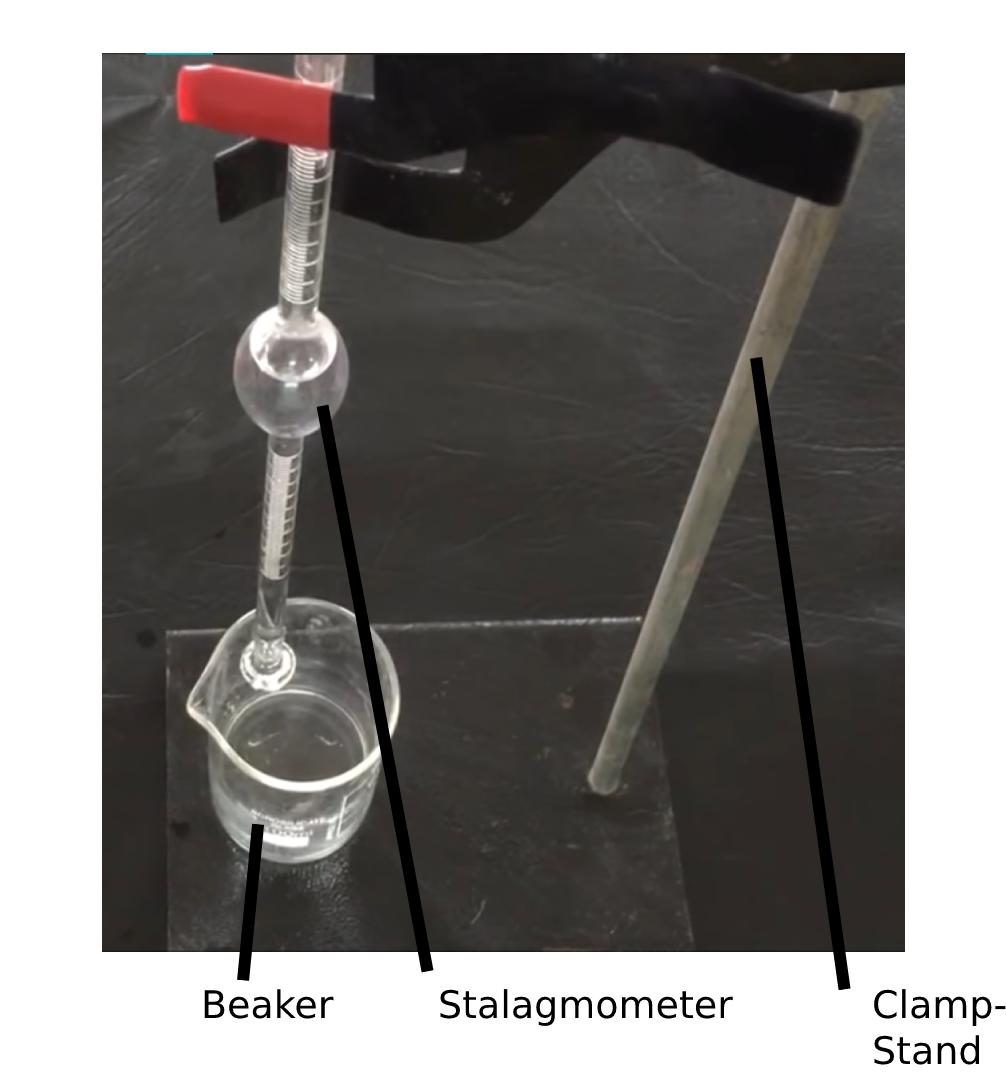
\includegraphics[width=5cm]{New Project (3).png}} }
    \caption*{Figure 2: Experimental Set-Up}%
    \label{fig:example}%
\end{figure}
\FloatBarrier

\subsection{Procedure}

\subsubsection{Risk Assessment}

\par{I wore gloves, a face-shield, safety goggles and a lab coat as the salt powder (potassium sulphate in particular) are an irritant if inhaled through the nose or absorbed through the skin or eye.}

\subsubsection{Ethical Considerations}

\par{There were no ethical issues in the experiment due to it's nature. There was also minimal wastage of solutions as only the necessary amount of readings were taken and thus, no extra solutions were prepared}

\subsubsection{Environmental Considerations}

\par{No harm was done to the environment and I ensured to dispose of all the chemicals used in a chemical disposal bin.}

\subsubsection{Preparation of Salts}
    \begin{enumerate}
        \item Using equations 3 and 4 (below), I calculated the mass of lithium sulphate needed to be dissolved in 300ml of water to get a concentration of 1 mol/$dm^3$.
        \begin{equation}
        \text{Mole} = \text{Concentration} \times \text{Volume}    
        \end{equation}
        \begin{equation}
        \text{Mass} = \text{Molar~Mass} \times \text{Number~of~Moles}
        \end{equation}
        \item Placing the beaker onto a weighing balance and using a spatula, I added the calculated the mass of lithium sulphate to the water.
        \item I stirred the solution of lithium sulphate and water vigorously using a stirring rod
        \item I repeated steps 1-3 for sodium sulphate
        \item I repeated steps 1-3 for potassium sulphate
        \item I repeated steps 1-3 for beryllium sulphate
        \item I repeated steps 1-3 for magnesium sulphate
        \item I repeated steps 1-3 for calcium sulphate
        \item I repeated steps 1-3 for sodium acetate
        \item I repeated steps 1-3 for potassium acetate
    \end{enumerate}


\subsubsection{Experimental Procedure}

\begin{enumerate}
\vspace{-0.5cm}
    \item I measured the mass ($\textt{M_{grav}}$) of the empty gravity bottle on the weighing balance 
    \item Next, I mounted a clean and dry stalagmometer on the clamp 
    \item Then I filled a beaker (300ml) with distilled water. The bottom end of the stalagmometer was immersed in the beaker and was sucked so that the water is above the bulb and on the fill line
    \item I observed the stalagmometer until 20 drops of water was collected in the gravity bottle
    \item I weighed the gravity bottle with the drops of water ($M_{grav}+M_{water} &= M_{total}$)
    \item I emptied and dried the gravity bottle and stalagmometer were and prepared them for the next experiment
    \item I repeated steps 2-6 5 times
    \item I repeated steps 2-7 for lithium sulphate
    \item I repeated steps 2-7 for sodium sulphate
    \item I repeated steps 2-7 for potassium sulphate
    \item I repeated steps 2-7 for beryllium sulphate
    \item I repeated steps 2-7 for magnesium sulphate
    \item I repeated steps 2-7 for calcium sulphate
    \item I repeated steps 2-7 for sodium acetate
    \item I repeated steps 2-7 for potassium acetate
\end{enumerate}

\subsection{Data Collection}

\begin{longtable}[c]{|c|c|c|c|c|c|}
\caption{Mass of water and various aqueous salt solutions at 35°C }
\label{tab:my-table}\\
\hline
\multirow{2}{*}{\textbf{Liquid}} & \multicolumn{5}{c|}{\textbf{Mass (g) ± 0.01g}}                                               \\ \cline{2-6} 
                                 & \textbf{Trial 1} & \textbf{Trial 2} & \textbf{Trial 3} & \textbf{Trial 4} & \textbf{Trial 5} \\ \hline
\endfirsthead
%
\multicolumn{6}{c}%
{{\bfseries Table \thetable\ continued from previous page}} \\
\hline
\multirow{2}{*}{\textbf{Liquid}} & \multicolumn{5}{c|}{\textbf{Mass (g) ± 0.01g}}                                               \\ \cline{2-6} 
                                 & \textbf{Trial 1} & \textbf{Trial 2} & \textbf{Trial 3} & \textbf{Trial 4} & \textbf{Trial 5} \\ \hline
\endhead
%
H₂O      & 0.99 & 1.01 & 1.00 & 0.99 & 1.00 \\ \hline
Li₂SO₄   & 1.99 & 2.00 & 2.01 & 1.98 & 2.01 \\ \hline
Na₂SO₄   & 1.75 & 1.77 & 1.75 & 1.76 & 1.76 \\ \hline
K₂SO₄    & 1.59 & 1.6  & 1.58 & 1.6  & 1.60 \\ \hline
BeSO₄    & 3.42 & 3.41 & 3.4  & 3.4  & 3.41 \\ \hline
MgSO₄    & 2.36 & 2.37 & 2.35 & 2.36 & 2.36 \\ \hline
CaSO₄    & 2.68 & 2.69 & 2.69 & 2.7  & 2.69 \\ \hline
CH₃COONa & 0.94 & 0.93 & 0.93 & 0.92 & 0.93 \\ \hline
CH₃COOK  & 0.91 & 0.90 & 0.91 & 0.92 & 0.91 \\ \hline
\end{longtable}

\subsection{Data Processing}

\par{Using the collected data, I was able to calculate the surface tension for each liquid. The absolute uncertainty in the mass was ±0.01g as the precision of the weighing scale used to measure the mass of the various solutions. I calculated the surface tension of each salt solution using equation 2. The reference liquid chosen was water. The surface tension for water, the reference liquid, was taken as 0.07035 J/$m^2$ using data from the Dortmund Data Bank\footnote{DDBST GmbH. “Surface Tension of Water from Dortmund Data Bank.” Dortmund Data Bank, DDBST GmbH, www.ddbst.com/en/EED/PCP/SFT$\_$C174.php.}. Before that, however, I would need to calculate the average mass of the of the solutions of each salt. I calculated this average by adding all of the collected mass values for a specific salt solution and then dividing the sum by 5. I calculated the uncertainty for the calculated surface tension by adding the relative uncertainty for the mass of water and the mass of the aqueous salt solution and then multiplying the sum of the relative errors with the calculated surface tension. However, as demonstrated in table 3, the relative error was smaller than random error for some of the salts (due to their greater mass) and as a result, the random error was used. This was calculated by calculating the range of the mass values for each solution. After performing these calculations, the following data would be obtained:}

\begin{longtable}[c]{|c|c|}
\caption{Mass of water and various salt solutions at 35°C}
\label{tab:my-table}\\
\hline
\textbf{Liquid} & \textbf{Average Mass (g) ± 0.01g} \\ \hline
\endfirsthead
%
\multicolumn{2}{c}%
{{\bfseries Table \thetable\ continued from previous page}} \\
\hline
\textbf{Liquid} & \textbf{Average Mass (g) ± 0.01g} \\ \hline
\endhead
%
H₂O             & 1.00                              \\ \hline
Li₂SO₄          & 2.00                              \\ \hline
Na₂SO₄          & 1.76                              \\ \hline
K₂SO₄           & 1.60                              \\ \hline
BeSO₄           & 3.41                              \\ \hline
MgSO₄           & 2.36                              \\ \hline
CaSO₄           & 2.69                              \\ \hline
CH₃COONa        & 0.93                              \\ \hline
CH₃COOK         & 0.91                              \\ \hline
\end{longtable}

\begin{longtable}[c]{|c|c|c|}
\caption{Relative and random errors for water and various aqueous salts}
\label{tab:my-table}\\
\hline
\textbf{Liquid} & \textbf{Relative Uncertainty in Surface Tension} & \textbf{Random Error} \\ \hline
\endfirsthead
%
\multicolumn{3}{c}%
{{\bfseries Table \thetable\ continued from previous page}} \\
\hline
\textbf{Liquid} & \textbf{Uncertainty in Surface Tension} & \textbf{Random Error} \\ \hline
\endhead
%
H₂O             & 0.010                                   & 0.010                 \\ \hline
Li₂SO₄          & 0.005                                   & 0.015                 \\ \hline
Na₂SO₄          & 0.006                                   & 0.010                 \\ \hline
K₂SO₄           & 0.006                                   & 0.010                 \\ \hline
BeSO₄           & 0.003                                   & 0.010                 \\ \hline
MgSO₄           & 0.004                                   & 0.010                 \\ \hline
CaSO₄           & 0.004                                   & 0.010                 \\ \hline
CH₃COONa        & 0.011                                   & 0.010                 \\ \hline
CH₃COOK         & 0.011                                   & 0.010                 \\ \hline
\end{longtable}

\begin{longtable}[c]{|c|c|c|}
\caption{Surface tension of water and various salt solutions at 35°C and their absolute uncertainties}
\label{tab:my-table}\\
\hline
\textbf{Liquid} & \textbf{Surface Tension (J/m²)} & \textbf{Absolute Uncertainty in Surface Tension (J/m²)} \\ \hline
\endfirsthead
%
\multicolumn{3}{c}%
{{\bfseries Table \thetable\ continued from previous page}} \\
\hline
\textbf{Liquid} & \textbf{Surface Tension (J/m²)} & \textbf{Absolute Uncertainty in Surface Tension (J/m²)} \\ \hline
\endhead
%
H₂O      & 0.07035 & -     \\ \hline
Li₂SO₄   & 0.140   & 0.004 \\ \hline
Na₂SO₄   & 0.124   & 0.002 \\ \hline
K₂SO₄    & 0.112   & 0.002 \\ \hline
BeSO₄    & 0.240   & 0.005 \\ \hline
MgSO₄    & 0.166   & 0.003 \\ \hline
CaSO₄    & 0.189   & 0.004 \\ \hline
CH₃COONa & 0.065   & 0.001 \\ \hline
CH₃COOK  & 0.064   & 0.001 \\ \hline
\end{longtable}

\subsection{Sample Calculations}

\par{The mass of lithium sulphate salt added to the water was calculated as follows:}

\begin{equation*}
        \text{Mole} = 1 mol/dm^3 \times 0.3 dm^3 = 0.3 mol
\end{equation*}

\begin{equation*}
    \text{Mass} = 0.3 mol \times 109.94 g/mol = 32.98 g
\end{equation*}

\par{The average mass for lithium sulphate was calculated as follows:}

\begin{equation*}
    Mass_{ave} &= \sum_{n=1}^{5} \text{Mass} = \frac{1.99+2.00+2.01+1.98+2.01}{5} \approx \text{2.00 g}
\end{equation*}

\par{The surface tension for lithium sulphate was calculated as follows:}

\begin{equation*}
    \sigma_{Li_2SO_4} = \frac{2}{\frac{1}{0.07035}} = 0.140 J/m^2 
\end{equation*}

\par{The relative uncertainty for lithium sulphate was calculated as follows: }

\begin{equation*}
    \Delta \text{Mass} = \frac{0.01}{2} = 0.005 
\end{equation*}

\par{The relative uncertainty for lithium sulphate was calculated as follows: }

\begin{equation*}
    Mass_{random} = \frac{2.01-1.98}{2} = 0.015 
\end{equation*}

\par{The absolute error for the surface tension was calculated as follows:}

\begin{equation*}
    \Delta \sigma = (0.015 + 0.01) \times 0.140 = 0.004 J/m^2
\end{equation*}

\par{With the data in table 4, a graph of surface tension against the salts can be plotted, which yields the following graph:}

\begin{center}
    \includegraphics[scale=0.85]{rishabh.png}
    \par{Graph 1: Surface tension of water and various aqueous salt solutions against the solutions}
\end{center}

\section{Conclusion and Evaluation}

\subsection{Conclusion}

\par{After the data was collected and processed, I concluded that the results support the hypothesis: organic salts do decrease the surface tension of water, while inorganic salts increase the surface tension. One can observe both graph 1 and table 4 and notice that the inorganic salt solutions all had higher surface tensions than water, while the organic salt solutions had lower surface tensions than water. Hence organic salts reduce the surface tension of water while inorganic salts increase it. There were no anomalies for these trends. Nevertheless, the hypothesis predicted a strong relationship between the decrease in surface tension and addition of organic salts, while the organic salts did not reduce the surface tension by a large amount. This may have been due to using acetate salts, which have weak anions and thus does not significantly  break the strong polar bonds in water. This would be discussed more thoroughly in the evaluation. On the other hand, the error bars were insignificant, thus, the precision was  high. This could be attributed to the fact that no more than necessary measurements were taken. I took a total of 5 trials for each aqueous salt solution and most of the readings lied between the expected values with a range of 0.01g. Additionally, the instruments used were also highly accurate as the mass was measured using a digital weighing balance.}

\subsection{Evaluation}

\subsubsection{Strengths}

% Please add the following required packages to your document preamble:
% \usepackage{longtable}
% Note: It may be necessary to compile the document several times to get a multi-page table to line up properly
\begin{longtable}[c]{|c|c|}
\caption{}
\label{tab:my-table}\\
\hline
\textbf{Strengths} &
  \textbf{Evidence} \\ \hline
\endfirsthead
%
\multicolumn{2}{c}%
{{\bfseries Table \thetable\ continued from previous page}} \\
\hline
\textbf{Strengths} &
  \textbf{Evidence} \\ \hline
\endhead
%
\begin{tabular}[c]{@{}c@{}}Large number of inorganic salts used: Due to using a large\\ number of inorganic salts, the trend for the inorganic salts \\ increasing surface tension became more reliable.\end{tabular} &
  \begin{tabular}[c]{@{}c@{}}All 6 inorganic salts resulted in the surface tension\\ of water decreasing. This suggests that inorganic\\ salts increase surface tension of water.\end{tabular} \\ \hline
\begin{tabular}[c]{@{}c@{}}Number of trials: Due to doing 5 trials of measuring the \\ mass for each salt, the random error associated with\\ measuring the mass of the solutions was small. This\\ meant that the trend were reliable.\end{tabular} &
  The error bars for the data were insignificant \\ \hline
\begin{tabular}[c]{@{}c@{}}Drop Weight Method: The experimental procedure itself\\ was extremely well suited to measuring the surface tension \\ of each aqueous salt solution and the digital scale could \\ measure the mass of all samples with low random error\end{tabular} &
  \begin{tabular}[c]{@{}c@{}}The accuracy and precision of the experiment were \\ high. Not only were the error bars insignificant, \\ suggesting low random error and systemic\\ error, but the trends remained consistent for\\ all samples.\end{tabular} \\ \hline
\end{longtable}

\subsubsection{Limitations}

% Please add the following required packages to your document preamble:
% \usepackage{longtable}
% Note: It may be necessary to compile the document several times to get a multi-page table to line up properly
\begin{longtable}[c]{|c|c|c|}
\caption{}
\label{tab:my-table}\\
\hline
\textbf{Limitations} & \textbf{Significance} & \textbf{Improvement} \\ \hline
\endfirsthead
%
\multicolumn{3}{c}%
{{\bfseries Table \thetable\ continued from previous page}} \\
\hline
\textbf{Limitations} & \textbf{Significance} & \textbf{Improvement} \\ \hline
\endhead
%
\begin{tabular}[c]{@{}c@{}}Low number of organic salts used: Due \\ to using a low number of organic salts, \\ the trend for the organic salts decreasing \\ surface tension was less reliable\\ than the trend for the inorganic salts.\end{tabular} &
  \begin{tabular}[c]{@{}c@{}}High significance because the trend \\ for organic salts may only be true \\ for group 1 acetates and thus the \\ conclusion may have been \\ extrapolated from a small set of data.\end{tabular} &
  \begin{tabular}[c]{@{}c@{}}Use more organic salts such as\\ group 2 acetates, oxalates, \\ urates and phosphinates.\end{tabular} \\ \hline
\begin{tabular}[c]{@{}c@{}}Low variety of salts used: Due to \\ using only sulphates and\\ acetates as other salts were unavailable, \\ the trend for both \\ organic and inorganic salts \\ may be unreliable.\end{tabular} &
  \begin{tabular}[c]{@{}c@{}}High significance as the observed \\ trends may be as a result of\\ properties of sulfates\\ and acetates (sulfates are highly \\ hydrophilic while acetates are not)\\ and not due to the salt being \\ organic or inorganic\end{tabular} &
  \begin{tabular}[c]{@{}c@{}}Use different types of surfactants\\ and inorganic and organic salts\\ such as group 1, 2 and 3 halides\\ and hydroxides, ethoxylates, \\ or amino oxides\end{tabular} \\ \hline
\begin{tabular}[c]{@{}c@{}}Concentrations of salts: The concentration\\  of salts were kept constant at 1 mol/dm³.\\  This may reduce the reliability of the \\ trends as greater or lower \\ concentrations of salts \\ may reveal a different trend.\end{tabular} &
  \begin{tabular}[c]{@{}c@{}}Medium significance as, while a \\ different trend may be revealed \\ at different concentrations,\\ this is unlikely because \\ properties of salts are unlikely to \\ change at higher concentrations.\end{tabular} &
  \begin{tabular}[c]{@{}c@{}}Use a range of concentrations of \\ salt such as from 0 mol/dm³ to \\ 5 mol/dm³ with intervals of \\ 0.25 mol/dm³.\end{tabular} \\ \hline
\end{longtable}

\subsubsection{Scope}

\par{This experiment can be extended to observe the effect of inorganic and organic salts on the surface tension of different solvents such as n-heptane, ethanol, or cyclohexane. The independent and dependent variables would remain the same in that case. Such an experiment would be valuable to the real world as identifying the measures to affect surface tension for these industrial solvents may result in cheaper industrial processes or higher quality products.}

\par{Secondly, this experiment could also be extended to observe the effects of different polar heads on the surface tension of different solvents. In that case, the independent variable would be the polar heads, which can be cations, non-ionic or anions and the dependent variable would be the surface tension of the solvents. Such an experiment may reveal other properties of salts that affect surface tension.}

\par{Finally, this experiment can be extended to observe the effect of temperature on surface tension of different solvents. The independent variable would be temperature and the dependent variable would be surface tension.}

\pagebreak

\section{Bibliography}

\hspace{-1.3cm}
Bustos,  Elsa  Susana  Sep ́ulveda.“Surface  Tension.”  Surface  Tension  and  Capillarity,  University  of  Florida,  2004,fsz.ifas.ufl.edu/surfacetensionandcapillarity/html/entension.htm
\newline \\
DDBST  GmbH.  “Surface  Tension  of  Water  from  Dortmund  Data  Bank.”  Dortmund  Data  Bank,  DDBST  GmbH,www.ddbst.com/en/EED/PCP/SFTC174.php
\newline \\
Petrucci, Ralph H., et al.  General Chemistry:  Principles and Modern Applications.  Upper Saddle River, NJ: Prentice Hall,2017.
\newline \\
Science  Buddies.“Measuring  Surface  Tension  of  Water  with  a  Penny  —  Science  Project.”  Science  Buddies,   20Nov.2020,  www.sciencebuddies.org/science-fair-projects/project-ideas/Chemp021/chemistry/measuring-surface-tension-of-water-with-a-penny#background.


\end{document}
